\documentclass{beamer}
\usetheme{Boadilla}
\usepackage[labelformat=empty]{caption}
\usepackage{tikz}
\usepackage{graphicx}

\usetikzlibrary{positioning}
\usepackage{media9}

\title[Piston Problem]{}
\subtitle{}
\author[Monisha Muralidharan M]{}
\institute[]{\scriptsize }
\date{\tiny \today}

\begin{document}


\begin{frame}{Piston Problem}
    \scriptsize{
    \begin{minipage}{0.4\textwidth}
       
     Time harmonic $e^{-i\omega t}$
    \begin{figure}
        \centering
        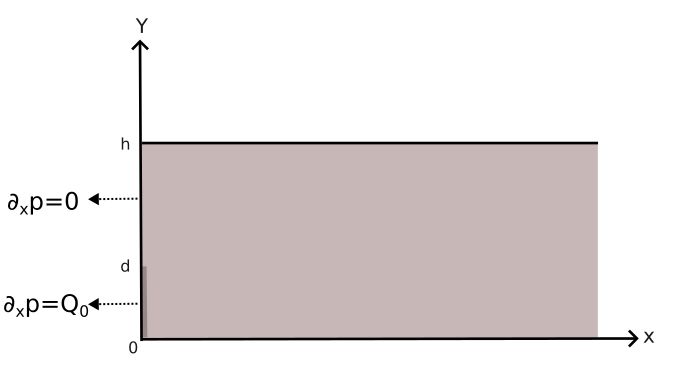
\includegraphics[width=1\textwidth]{piston.png} 
    \end{figure}
    \end{minipage}
    \begin{minipage}{0.55\textwidth}

        A semi-infinite waveguide along x bounded at x=0 has a height h in the y direction.
        A piston is located at x=0 and occupies y=[0,d] with the following boundary conditions,\\
        $\partial_xp=Q_0 \in x=0, y=[0,d]$,\\
        $\partial_xp=0 \in x=0, y=[d,h]$,\\
        $\partial_yp=0 \in x>0, y=0,h$.\\
        
        

         \end{minipage}
        The normal derivative of the pressure on the walls of the waveguide is zero.\\
        The normal derivative of the pressure on the piston is $Q_0$.
        Solving the Helmholtz equation $(\nabla +k^2)p=0$ for the pressure field p in the waveguide,
        and considering only the outgoing wave condition \[ p(x,y)=\sum_{n=0}^{\infty}A_n e^{ik_nx} g_n(y)\]. Where, \quad$g_n(y)=\sqrt{\frac{\epsilon}{h}}\cos(\frac{n\pi}{h}y)$, $\epsilon=2-\delta_{0n}$, $k_n=\sqrt{k^2-(\frac{n\pi}{h})^2}$.
        \\Find $A_n$ and reconstruct the pressure field.
    }
\end{frame}

 \begin{frame}
Considering only the forward going wave,
\[ p(x,y)=\sum_{n=0}^{\infty}A_n e^{ik_nx} g_n(y),\] 
The pressure derivative at x=0 is given by,
\[\partial_xp(0,y)=\sum_{n=0}^{\infty}ik_nA_n g_n(y),\]
Using the orthogonality of $g_n(y)$, we get
\[\int_0^h \partial_xp(0,y)g_m(y)dy=\int_{0}^{h}\sum_{n=0}^{\infty}ik_nA_n g_n(y)g_m(y) dy,\]

\[\int_{0}^{h}\sum_{n=0}^{\infty}ik_nA_n g_n(y)g_m(y) dy= \int_0^d Q_0 g_m(y)dy + \int_{d}^{h}0 dy,\]

\[ik_mA_m=\int_0^d Q_0 g_m(y)dy,\]

 \end{frame}

 \begin{frame}

\[A_m=\frac{-iQ_0}{k_m}\int_0^d g_m(y)dy,\]
\[A_m=\frac{-iQ_0}{k_m}\int_0^d \sqrt{\frac{\epsilon}{h}}\cos(\frac{m\pi}{h}y)dy,\]
\[A_m=\frac{-iQ_0}{k_m}\sqrt{\frac{\epsilon}{h}}\frac{h}{m\pi}\sin(\frac{m\pi}{h}d).\]
For m$>$0\[A_m=\frac{-iQ_0 d}{k_m}\sqrt{\frac{2}{h}}\operatorname{sinc}(\frac{m\pi}{h}d).\] 
For m=0   \[A_0=\frac{-iQ_0 d}{k_0}\sqrt{\frac{1}{h}}.\]       
\\
\begin{minipage}{0.25\textwidth}
\[\bold{A}=\begin{bmatrix}A_0\\ A_1\\ :\\ A_m\\ \end{bmatrix}\] 
\end{minipage}
\hfill
\begin{minipage}
{0.6\textwidth}
Where, $A_m=  \frac{-iQ_0 d}{k_m}\sqrt{\frac{2-\delta_{0m}}{h}}\bold{\operatorname{sinc}}{(\frac{m \pi d}{h})} .$\end{minipage}
 \end{frame}
\begin{frame}
The pressure field in the waveguide is given by,
\[p(x,y)=\sum_{n=0}^{\infty}A_n e^{ik_nx} g_n(y),\]
\[p(x,y)=\sum_{n=0}^{\infty}\frac{-iQ_0 d}{k_n}\sqrt{\frac{2-\delta_{0n}}{h}}\operatorname{sinc}(\frac{n\pi}{h}d) e^{ik_nx} \sqrt{\frac{2-\delta_{0n}}{h}}\cos(\frac{n\pi}{h}y),\]
\[p(x,y)=\frac{-iQ_0 d}{h}\sum_{n=0}^{\infty}\frac{2-\delta_{0n}}{k_n}\operatorname{sinc}(\frac{n\pi}{h}d) \cos(\frac{n\pi}{h}y)e^{ik_nx}.\]
\\
\end{frame}
\end{document}